% \usepackage{tikz}
\usetikzlibrary{trees}
% \usepackage{listings}
% \usepackage{xcolor}
% \usepackage{amsmath}

\lstset{
  basicstyle=\ttfamily\small,
  frame=single,
  backgroundcolor=\color{gray!10},
  breaklines=true,
  keywordstyle=\color{blue},
  commentstyle=\color{gray},
  stringstyle=\color{purple},
  showstringspaces=false
}

\subsection{Exercise 3 Sheet Solution (Spring 2025)}

\subsubsection{Q1. AVL Tree Construction}
Build an AVL tree with the following values: 15, 20, 24, 10, 13.

\textbf{Answer:}

\textbf{Step 1: Insert 15} \\
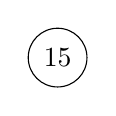
\begin{tikzpicture}[level distance=1.2cm, sibling distance=1.5cm, every node/.style={draw, circle}]
\node {15};
\end{tikzpicture}

\textbf{Step 2: Insert 20} \\
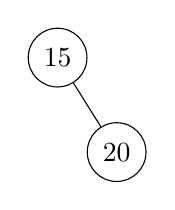
\begin{tikzpicture}[level distance=1.2cm, sibling distance=1.5cm, every node/.style={draw, circle}]
\node {15}
  child[missing]
  child {node {20}};
\end{tikzpicture}

\textbf{Step 3: Insert 24 → Left Rotation} \\
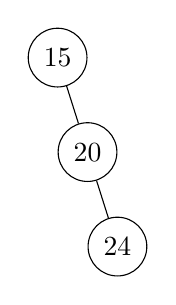
\begin{tikzpicture}[level distance=1.2cm, sibling distance=1.5cm, every node/.style={draw, circle}]
\node {15}
  child [right] {node{20} 
    child [right]{node{24}}
  }
  ;
\end{tikzpicture}
\quad
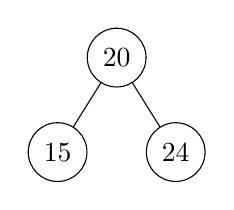
\begin{tikzpicture}[level distance=1.2cm, sibling distance=1.5cm, every node/.style={draw, circle}]
\node {20}
  child {node {15}}
  child {node {24}};
\end{tikzpicture}

\textbf{Step 4: Insert 10} \\
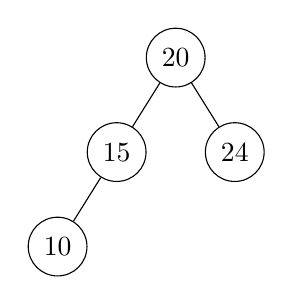
\begin{tikzpicture}[level distance=1.2cm, sibling distance=1.5cm, every node/.style={draw, circle}]
\node {20}
  child {
    node {15}
    child {node {10}}
    child [missing]
  }
  child {node {24}};
\end{tikzpicture}

\textbf{Step 5: Insert 13 → LR Rotation} \\
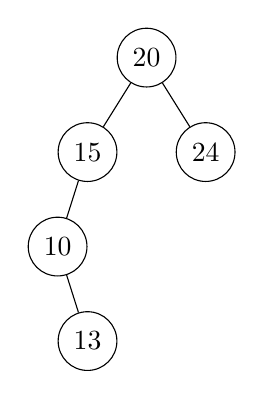
\begin{tikzpicture}[level distance=1.2cm, sibling distance=1.5cm, every node/.style={draw, circle}]
\node {20}
  child {node {15}
    child[left] {node {10}
      child [right] {node {13}}
    }
  }
  child {node {24}};
\end{tikzpicture}
\quad
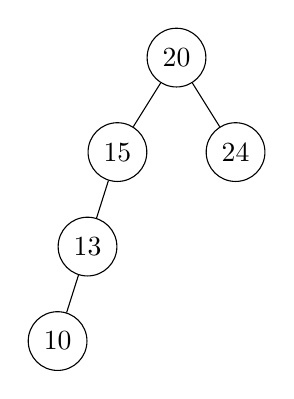
\begin{tikzpicture}[level distance=1.2cm, sibling distance=1.5cm, every node/.style={draw, circle}]
\node {20}
  child {node {15}
    child[left] {node {13}
      child [left] {node {10}}
    }
  }
  child {node {24}};
\end{tikzpicture}
\quad
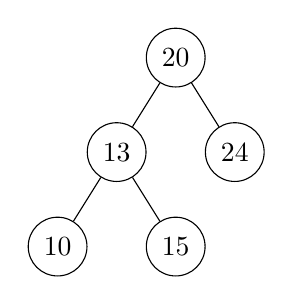
\begin{tikzpicture}[level distance=1.2cm, sibling distance=1.5cm, every node/.style={draw, circle}]
\node {20}
  child {
    node {13}
    child {node {10}}
    child {node {15}}
  }
  child {node {24}};
\end{tikzpicture}

\subsubsection{Q2. AVL Tree Deletion and Rotations}

\textbf{Delete 53 (Right Rotation)}

Initial tree:
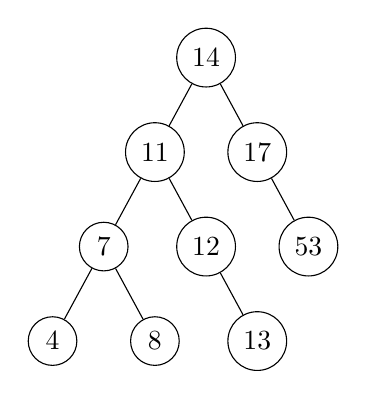
\begin{tikzpicture}[level distance=1.2cm, sibling distance=1.3cm, every node/.style={draw, circle}]
\node {14}
  child {
    node {11}
    child {node {7}
      child {node {4}}
      child {node {8}}}
    child {node {12}
      child[missing]
      child {node {13}}}
  }
  child {node {17}
    child[missing]
    child {node {53}}};
\end{tikzpicture}

After deleting 53 and applying right rotation:
\begin{lstlisting}
Left height = 3 (subtree rooted at 11)
Right height = 1 (subtree rooted at 17)
Balance factor = +2  left-heavy
Left child 11 had:
Balanced subtrees (so no double rotation needed)
Therefore, this is a Left-Left Case and a right rotation at 14 is the correct rebalancing operation.
Let me know if you'd like a visual step-by-step animation or code for this.
\end{lstlisting}

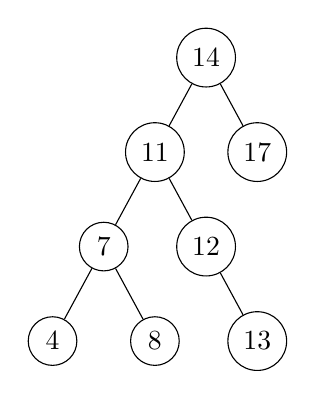
\begin{tikzpicture}[level distance=1.2cm, sibling distance=1.3cm, every node/.style={draw, circle}]
\node {14}
  child {
    node {11}
    child {node {7}
      child {node {4}}
      child {node {8}}}
    child {node {12}
      child[missing]
      child {node {13}}}
  }
  child {node {17}};
\end{tikzpicture}
\quad
\quad
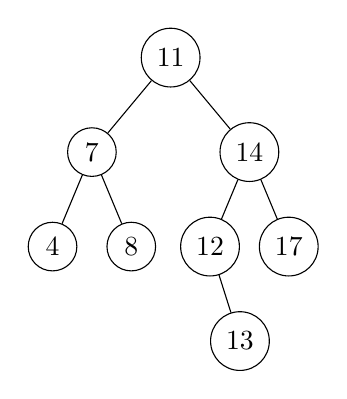
\begin{tikzpicture}[
  level distance=1.2cm, 
  sibling distance=1.0cm, 
  level 1/.style={sibling distance=2cm},
  level 2/.style={sibling distance=1cm},
  every node/.style={draw, circle}]
\node {11}
  child {
    node {7}
    child {node {4}}
    child {node {8}}
  }
  child {
    node {14}
    child {node {12}
      child[right] {node {13}}
    }
    child {node {17}}
  };
\end{tikzpicture}

\vspace{0.5cm}
\textbf{Delete 17 (LR Rotation)}

Initial tree: \\
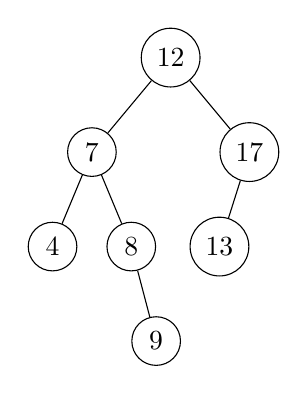
\begin{tikzpicture}[
  level distance=1.2cm, 
  sibling distance=1.0cm, 
  level 1/.style={sibling distance=2cm},
  level 2/.style={sibling distance=1cm},
  every node/.style={draw, circle}]
\node {12}
  child {
    node {7}
    child {node {4}}
    child {node {8}
      child[right]{node{9}}
    }
  }
  child {
    node {17}
    child[left] {node {13}}
  };
\end{tikzpicture}
After delete 17: \\
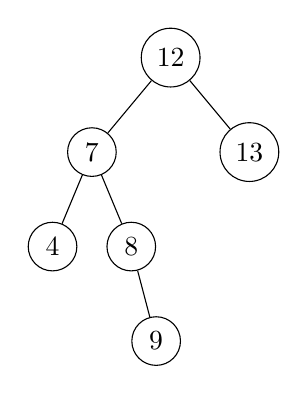
\begin{tikzpicture}[
  level distance=1.2cm, 
  sibling distance=1.0cm, 
  level 1/.style={sibling distance=2cm},
  level 2/.style={sibling distance=1cm},
  every node/.style={draw, circle}]
\node {12}
  child {
    node {7}
    child {node {4}}
    child {node {8}
      child[right]{node{9}}
    }
  }
  child {node {13}};
\end{tikzpicture}
After LR rotation: \\

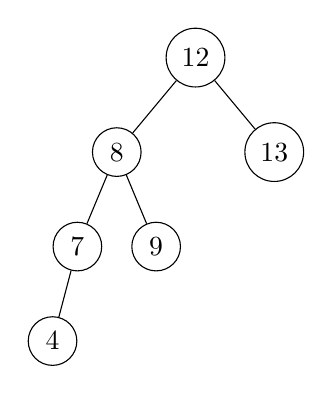
\begin{tikzpicture}[
  level distance=1.2cm, 
  sibling distance=1.0cm, 
  level 1/.style={sibling distance=2cm},
  level 2/.style={sibling distance=1cm},
  every node/.style={draw, circle}]
\node {12}
  child {
    node {8}
    child {node {7}
      child[left]{node{4}}
    }
    child {node {9}}
  }
  child {node {13}};
\end{tikzpicture}
\quad
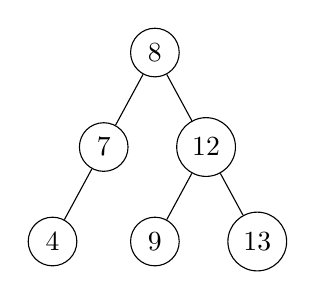
\begin{tikzpicture}[level distance=1.2cm, sibling distance=1.3cm, every node/.style={draw, circle}]
\node {8}
  child {
    node {7}
    child {node {4}}
    child[missing]
  }
  child {
    node {12}
    child {node {9}}
    child {node {13}}
  };
\end{tikzpicture}

\subsubsection{Q3. Time Complexity of Algorithms}

\textbf{1 Multiply all elements in the array}

\begin{lstlisting}
def product(arr):
    n = len(arr)
    x = 1
    i = 0
    while i < n:
        x *= arr[i]
        i += 1
    return x
\end{lstlisting}

\textbf{Answer:} $O(n)$

\textbf{2 Modify the last value}

\begin{lstlisting}
def modify(arr):
    if len(arr) == 0:
        raise Exception("Array is empty")

    last = arr[-1]
    if last < 0:
        last = -last

    arr[-1] = last
\end{lstlisting}

\textbf{Answer:} $O(1)$

\textbf{3 Find the largest (method 1, brute force)}

\begin{lstlisting}
def largest1(arr):
    n = len(arr)
    max_val = 0

    for i in range(n):
        is_largest = True
        for j in range(n):
            if arr[i] < arr[j]:
                is_largest = False
        if is_largest:
            max_val = arr[i]

    return max_val
\end{lstlisting}

\textbf{Answer:} $O(n^2)$

\textbf{4 Find the largest (method 2, single scan)}

\begin{lstlisting}
def largest2(arr):
    n = len(arr)
    max_val = 0

    if n == 0:
        return 0
    else:
        max_val = arr[0]
        for i in range(n):
            if arr[i] > max_val:
                max_val = arr[i]

    return max_val
\end{lstlisting}

\textbf{Answer:} $O(n)$

\textbf{5 Find the largest (method 3, via sort)}

\begin{lstlisting}
def largest3(arr):
    arr.sort()  # assume O(n log n)

    if len(arr) == 0:
        return 0
    else:
        last = arr[-1]
        return last
\end{lstlisting}

\textbf{Answer:} $O(n \log n)$

% \end{document}
